\documentclass[]{elsarticle} %review=doublespace preprint=single 5p=2 column
%%% Begin My package additions %%%%%%%%%%%%%%%%%%%
\usepackage[hyphens]{url}

  \journal{An Elsevier journal} % Sets Journal name


\usepackage{lineno} % add
\providecommand{\tightlist}{%
  \setlength{\itemsep}{0pt}\setlength{\parskip}{0pt}}

\usepackage{graphicx}
\usepackage{booktabs} % book-quality tables
%%%%%%%%%%%%%%%% end my additions to header

\usepackage[T1]{fontenc}
\usepackage{lmodern}
\usepackage{amssymb,amsmath}
\usepackage{ifxetex,ifluatex}
\usepackage{fixltx2e} % provides \textsubscript
% use upquote if available, for straight quotes in verbatim environments
\IfFileExists{upquote.sty}{\usepackage{upquote}}{}
\ifnum 0\ifxetex 1\fi\ifluatex 1\fi=0 % if pdftex
  \usepackage[utf8]{inputenc}
\else % if luatex or xelatex
  \usepackage{fontspec}
  \ifxetex
    \usepackage{xltxtra,xunicode}
  \fi
  \defaultfontfeatures{Mapping=tex-text,Scale=MatchLowercase}
  \newcommand{\euro}{€}
\fi
% use microtype if available
\IfFileExists{microtype.sty}{\usepackage{microtype}}{}
\bibliographystyle{elsarticle-harv}
\usepackage{graphicx}
% We will generate all images so they have a width \maxwidth. This means
% that they will get their normal width if they fit onto the page, but
% are scaled down if they would overflow the margins.
\makeatletter
\def\maxwidth{\ifdim\Gin@nat@width>\linewidth\linewidth
\else\Gin@nat@width\fi}
\makeatother
\let\Oldincludegraphics\includegraphics
\renewcommand{\includegraphics}[1]{\Oldincludegraphics[width=\maxwidth]{#1}}
\ifxetex
  \usepackage[setpagesize=false, % page size defined by xetex
              unicode=false, % unicode breaks when used with xetex
              xetex]{hyperref}
\else
  \usepackage[unicode=true]{hyperref}
\fi
\hypersetup{breaklinks=true,
            bookmarks=true,
            pdfauthor={},
            pdftitle={Do Drivers Dream of Walking? An Investigation of Travel Mode Dissonance from the Perspective of Subjective Wellbeing},
            colorlinks=false,
            urlcolor=blue,
            linkcolor=magenta,
            pdfborder={0 0 0}}
\urlstyle{same}  % don't use monospace font for urls

\setcounter{secnumdepth}{0}
% Pandoc toggle for numbering sections (defaults to be off)
\setcounter{secnumdepth}{0}
% Pandoc header
\usepackage{booktabs}
\usepackage{longtable}
\usepackage{array}
\usepackage{multirow}
\usepackage{wrapfig}
\usepackage{float}
\usepackage{colortbl}
\usepackage{pdflscape}
\usepackage{tabu}
\usepackage{threeparttable}
\usepackage{threeparttablex}
\usepackage[normalem]{ulem}
\usepackage{makecell}
\usepackage{xcolor}



\begin{document}
\begin{frontmatter}

  \title{Do Drivers Dream of Walking? An Investigation of Travel Mode Dissonance
from the Perspective of Subjective Wellbeing}
    \author[Some University]{Author 1\corref{c1}}
   \ead{a1@university.com} 
   \cortext[c1]{Corresponding Author}
    \author[Some School]{Author 2}
   \ead{a2@school.com} 
  
      \address[Some University]{Department, Street, City, State, Zip}
    \address[Some School]{Department, Street, City, State, Zip}
  
  \begin{abstract}
  Transportation in most of the world has been dominated for decades by a
  fascination with the automobile. Nonetheless, there is an increasing
  recognition that to achieve a variety of economic, environmental, and
  public health policy goals it is important to attract and retain active
  travelers and users of public transportation. A challenge with the way
  transportation policy is developed, however, is that it tends to focus
  on utilitarian considerations, which may miss other potential aspects of
  transportation that users value. In particular, subjective wellbeing
  (SWB) has been proposed as a way to enhance our understanding of the
  preferences and choices of travellers, as well as a way to evaluate the
  benefits of transportation beyond utilitarian considerations. The
  objective of this paper is to analyze the modes that people commonly
  use, and to what extent they are aligned (or not) with a variety of
  affective values associated with SWB. In other words, we are interested
  in the potential for dissonance with respect to the primary mode of
  travel, from the perspective of affective values. The study is based on
  data collected from a sample of travellers in the city of Santiago, in
  Chile. Participants in the study were asked about their usual mode of
  travel, and then were asked to name the mode or modes that they
  associate with the affective values of freedom, enjoyment, happiness,
  poverty, luxury and status. The results indicate that users of public
  transportation experience the most dissonance in terms of affective
  values, and active travellers the least. For those travellers who
  experience dissonance, active travel is the mode most commonly
  associated with freedom, enjoyment, and happiness, public transportation
  is most commonly associated with poverty, and the automobil is most
  commonly associated with luxury and status.
  \end{abstract}
  
 \end{frontmatter}

\hypertarget{introduction}{%
\section{1. Introduction}\label{introduction}}

Transportation planning for decades has focused on providing mobility
for the private automobile. This is a model of development that was
initially introduced in North America as a solution to problems created
by rapid urbanization, and that was eventually copied elsewhere
(Angotti, 1996; Brown et al., 2009). Despite the initial promise of
automotive technology, it is now evident that mobility centred on the
private automobile has given rise to a litany of maladies that are in
urgent need of correction. This includes environmental concerns (i.e.,
climate change; Chapman, 2007) as well as numerous other social
(Boschmann and Kwan, 2008; Lucas, 2019, 2012), health (Khreis et al.,
2016; Milne, 2012), and equity issues (Bocarejo and Oviedo, 2012;
Martens et al., 2012; Pereira et al., 2017).

As the real impacts of our societal dependence on the private
autombobile have become increasingly evident, the transportation agenda
has aimed to shift focus to the reduction of car use and towards the
creation of mobility polycultures that offer a broader menu of
transportation alternatives than primarily (or even just) the private
automobile (Miller, 2011). In order to successfully achieve this goal,
it is essential not only to provide the services and facilities that
support public transportation and active travel, but also to attract new
users to these modes of transportation (Ettema et al., 2011). Within
this context, it has been argued that sustainable transportation
policies require all participants in the transportation system to
challenge what Gossling and Cohen (2014) termed \emph{transportation
taboos}: deep-seated ideas concerning the contribution to emissions by
individuals, the inequality of market-based approaches, and the social
and psychological functions of transportation. With respect to the
latter, it is important to move beyond a purely utilitarian focus if we
are to understand how the affective value of the transportation
experience can be leveraged to improve alternative transportation -
particularly transit and active modes (Anable and Gatersleben, 2005;
Domarchi et al., 2008; Gatersleben and Uzzell, 2007; Steg, 2005).

A useful lens to investigate the social and psychological functions of
transportation is by means of the concept of subjective wellbeing (SWB;
see, inter alia, De Vos et al., 2013; and Chatterjee et al., 2019). SWB
is defined by the OECD as ``{[}g{]}ood mental states, including all of
the various evaluations, positive and negative, that people make of
their lives, and the affective reactions of people to their
experiences'' (\textbf{OECD, 2013, p.~10}). As memorably put by Steg
(2005): is the use of car a must, or is it a lust? A close alignment, or
consonance, between affective values and the mode of transportation used
to travel can result in greater subjective wellbeing and increase the
probability of choosing that mode (i.e., by satisfying the \emph{lust});
on the other hand, dissonance, that is, the lack of concordance between
the mode used and affective values would be detrimental to subjective
wellbeing, especially of those for whom the use of the mode is a
\emph{must} (De Vos, 2019; Mokhtarian and Pendyala, 2018). With these
considerations in mind, one aim of the present research is to
investigate \emph{who} experiences dissonance with respect to their
primary mode of travel and affective values, namely freedom, enjoyment,
happiness, feelings of poverty, luxury, and status. Furthermore, it is
possible, even if use of a particular mode is a \emph{must}, that
travellers may still \emph{lust} for something else - in other words,
the grass may in fact look greener from the window of the car. For this
reason, we also aim to investigate which mode or modes are most commonly
associated with affective values, with a focus on those travellers who
experience dissonance in their primary mode.

Research is based on data collected from a sample of travellers in the
city of Santiago in Chile. Survey respondents were asked about their
primary mode of travel, and also about the mode or modes that they
associate with the affective values mentioned above. The paper
contributes to the literature in three ways, as follows:

\begin{enumerate}
\def\labelenumi{\arabic{enumi}.}
\item
  The research reported here contributes to an emerging literature on
  the topic of transportation and affective values in the context of the
  Global South (Al-Ayyash and Abou-Zeid, 2019; Bejarano et al., 2017;
  Shao and Liang, 2019; Van et al., 2014; Zorrilla et al., 2019); to the
  best of our knowledge, the case of Chile has not yet been reported.
\item
  Although there is an extensive literature on the enjoyment of commute
  and other affective values (see for instance Paez and Whalen, 2010;
  Redmond and Mokhtarian, 2001; Whalen et al., 2013; Ye and Titheridge,
  2017), from a hedonic and even eudaimonic perspectives the analysis
  has yet to be applied more fully in terms of distributional issues --
  i.e.~which groups more commonly experience dissonance (see De Vos,
  2018).
\item
  The analysis shows the attitudes of people towards their primary mode
  and their perception towards `ideal modes' -- implying their
  preferences, even in situations when their ideal mode is not part of
  their actual choice set. More concretely, the results indicate that
  users of public transportation experience the most dissonance in terms
  of affective values, and active travellers the least. For those
  travellers who experience dissonance, active travel is the mode most
  commonly associated with freedom, enjoyment, and happiness, public
  transportation is most commonly associated with poverty, and the
  automobil is most commonly associated with luxury and status. We also
  find that there are some substantial variations in dissonance by age,
  education, income, and typical commute time. The attitudes of
  travellers towards transport modes are critical factors to be
  considered by policy-makers in case they want to promote and increase
  the use of public transport or active modes (Bornioli et al., 2019; De
  Vos et al., 2019; De Vos and Witlox, 2017; Garling et al., 2019;
  Redman et al., 2013).
\item ~
  \hypertarget{background}{%
  \section{Background}\label{background}}
\end{enumerate}

A consensus has emerged in the transportation community regarding the
need to complement the traditional utilitarian perspective of
transportation by looking at mobility and transport issues from the lens
of their affective functions. The affective value of transportation in
turn is important due to its potential to improve or detract from SWB.
One of the primary ways to explore this has been the satisfaction that
travelers feel towards their every day mobility experience (e.g.,
Cecilia Jakobsson Bergstad et al., 2011). As a consequence, there is a
wealth of research on satisfaction with the use of different modes of
transportation. For example, numerous studies report that car users
often have a higher level of satisfaction compared to other transport
modes (C. J. Bergstad et al., 2011; Eriksson et al., 2013; Redmond and
Mokhtarian, 2001; Whalen et al., 2013; but see Handy and Thigpen, 2019).
In a similar way, there are multiple reports that active travel also
tends to yield high levels of satisfaction (Gatersleben and Uzzell,
2007; Handy and Thigpen, 2019; Paez and Whalen, 2010; Smith, 2017;
St-Louis et al., 2014; Whalen et al., 2013), In contrast, public
transport users tend to assess their experience more negatively (Abenoza
et al., 2017; De Vos et al., 2016; Gatersleben and Uzzell, 2007; Handy
and Thigpen, 2019; Paez and Whalen, 2010). Multi-modal trips also
influence satisfaction levels; for instance, when an individual chooses
a particular mode of transportation, she will report a higher level of
satisfaction with that chosen mode -- perhaps as a form of \emph{post
hoc} validation (Susilo and Cats, 2014).

While the use of travel satisfaction has been mainly used in the context
of daily trips -- typically linked to cost-benefit and utilitarian
measurements --, the evaluation of Subjective Wellbeing (SWB) over time
has risen as an alternative measure. In the field of travel behaviour,
Ettema et al.~(2010, p. 725) define SWB as the degree to which an
individual positively evaluates the overall quality of their lives,
where the general life satisfaction encompasses a more extended
temporality -- which implies assuming a tendency to be more stable over
time. This concept has prompted a growing literature that complements
and applies SWB in a broader range of satisfaction scales and
situations. The definition of other factors such as travel choice mode,
attitudes and external elements of the built environment have been
studied for a broader understanding of the changes produced in the SWB
(e.g., Handy and Thigpen, 2019). As these factors do not necessarily
apply to the general life satisfaction on the long term, the studies
have aimed to determine both the direct and indirect effects on the
perception of users (see, e.g., Ye and Titheridge, 2017). Other concepts
have also emerged as the Satisfaction with Travel Scale (STS), a
measurement devised by Ettema et al.~(2011), as well as different scales
based on people's travel perceptions. De Vos et al.~(2015), for
instance, explore in detail the underlying dimensions of the affective
domain of STS on which SWB is based (for more on STS see also Friman et
al., 2013).

Recent literature on SWB and its link with transport have demonstrated a
relationship between people's perceptions and satisfaction with their
daily travel (e.g., Smith, 2017; Mokhtarian and Pendyala, 2018; St-Louis
et al., 2014). Scholars have shown that accessibility has been the most
developed factor that influences people's wellbeing (Delbosc, 2012), and
activities have a direct impact on travel satisfaction (Cecilia
Jakobsson Bergstad et al., 2011). Delbosc (2012, p. 28), for instance,
has summarised the most significant influences on psychological
wellbeing: poverty and employment, meaningful relationships and health.
However, understanding the components affecting people's perceptions
implies the differentiation between affective (also named as
symbolic-affective) and instrumental values (C. J. Bergstad et al.,
2011). Steg et al.~(2011) have compared symbolic-affective opposed to
instrumental-reasoned motives based on car-use, and other studies have
also found associations between affective and symbolic aspects of
car-use (see, e.g., Gatersleben and Uzzell, 2007; Lois and Lopez-Saez,
2009). Previous studies have also demonstrated how socio-demographic
factors affect the levels of SWB. The effect of income on SWB (Clark and
Oswald, 1996; Ferrer-i-Carbonell, 2005); education and unemployment
(Argyle et al., 1999); age (Diener and Eunkook Suh, 1997), and gender
(Tesch-Römer et al., 2008) have been extensively studied. Recent
research also suggests the links between commuting, SWB and emotional
wellbeing assessment (\textbf{Olson et al.~2013}; \textbf{Kahneman et
al.~2004}). However, more research is needed to understand how these
socio-demographic variables connect as well with the affective responses
to mode of travel (St-Louis et al., 2014).

The research needs already recognized in the developed world are also
markedly acute in the context of the Global South, where historical
inequality has tended to create a symbolic attachment to the automobile,
in addition to negative connotations for public transport and active
travel (Zorrilla et al., 2019). In this way, there is an emerging
literature that investigates affective factors in travel behaviour in a
number of developing countries. A cross-country study in Asia revealed
that the affective factors of public transportation and car use are
important, and in particular the social orderliness of transit was
suggested as a way to make this mode more attractive to users (Van et
al., 2014). In terms of active travel, a study in China found that
attitudes that embrace new styles and technologies despite their cost
are associated with the intention to continue using shared bicycles
(Shao and Liang, 2019). The importance of affective factors for policy
and planning is further highlighted by research in Colombia that shows
how users felt proud using a bicycle shared system, in addition to
experiencing feelings of belonging to a civic culture and the enjoyment
and pleasure of travel itself (Bejarano et al., 2017). This paper
contributes to further our understanding of affective values in travel
behaviour in a developing country.

\hypertarget{data-and-methods}{%
\section{3. Data and Methods}\label{data-and-methods}}

\hypertarget{context}{%
\section{3.1 Context}\label{context}}

Words to describe Santiago go here.

\hypertarget{sample}{%
\section{3.2 Sample}\label{sample}}

The study is based on a survey conducted in the city of Santiago during
the months of November and December 2016, that is, the end of the Spring
and beginning of Summer. The survey collected information on a wide
range of travel and related issues. The data collection considered a
quota-sampling method for gathering the information, considering the
socio-demographic information from Pre-Census of 2012. An equal
representation of both genders and a representation of the proportion of
inhabitants per area were chosen as relevant characteristics of the
sample. In total, there were \(n=451\) valid surveys, although not every
survey was complete and there were missing responses for some answers.

The survey was structured in eight sections, as follows: 1) Individual
characteristics of respondent; 2) Health; 3) Feelings and emotions; 4)
Reasons for travel and planning travel; 5) Social interaction; 6) Nature
and sustainability; 7) Information and telecommunications; 8) Built
environment; and 9) Commuting. For the present study, we draw data from
sections 1), 3) and 9). In terms of individual characteristics of the
respondents and their commute, participants were asked about basic
socio-demographic information, including age, level of education,
income, and the typical duration of their regular commute. The
descriptive statistics of the sample appear in Figure
\ref{fig:descriptive-statistics}. The sample tends to be younger, and
well-educated, with an almost uniform distribution of income levels. The
trend in typical commute time is towards longer commutes.

\begin{figure}
\centering
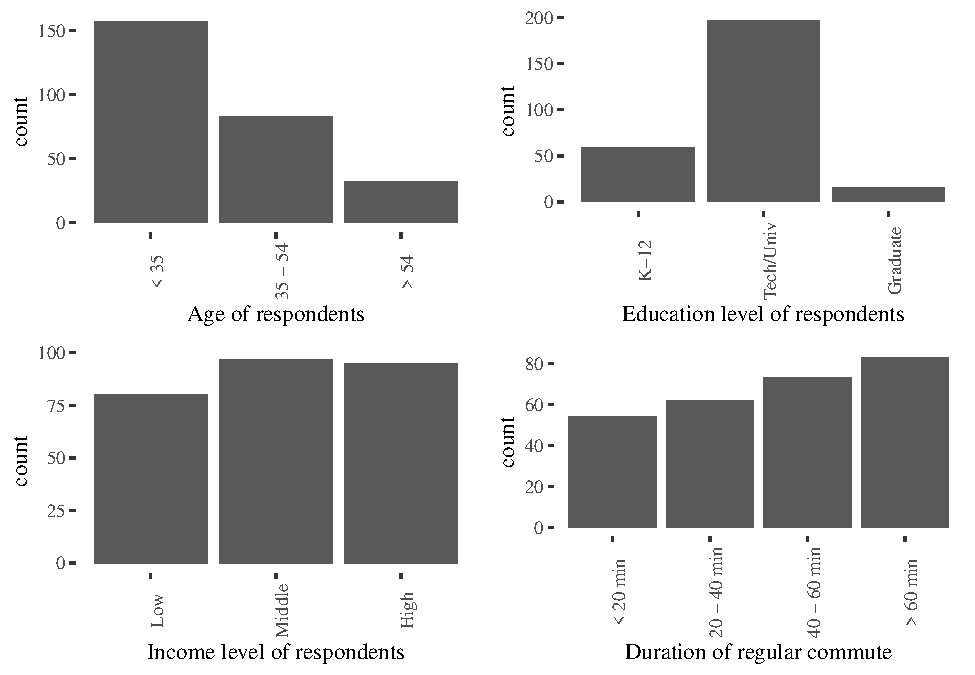
\includegraphics{Dissonance_Santiago_v1_files/figure-latex/plot-descriptive-statistics-1.pdf}
\caption{\label{fig:descriptive-statistics}Descriptive statistics of the
sample}
\end{figure}

In addition, respondents were asked about their primary mode of travel
for their regular commute. The modes available were Car, Taxi, Colectivo
(a form of shared ride, intermediate in flexibility and capacity between
taxi and bus); Motorcycle; Metro; Bus; Bicycle; Walking. As seen in the
top panel of Figure \ref{fig:primary-mode-travel}, the three most common
modes of travel are Metro, Bus, and Car, followed by Walking and Biycle.
For the analysis, we aggregate these modes into the following categories
(bottom panel of Figure \ref{fig:primary-mode-travel}): Car, Active
(Walking + Bicycle), Public (Metro + Bus), and Other (Taxi + Colectivo +
Motorcycle).

\begin{figure}
\centering
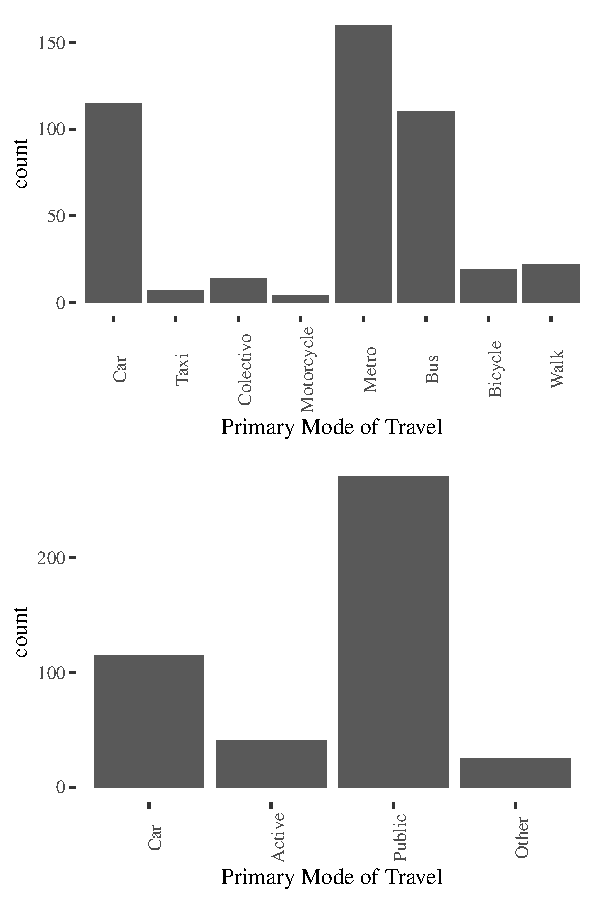
\includegraphics{Dissonance_Santiago_v1_files/figure-latex/figure-primary-mode-travel-1.pdf}
\caption{\label{fig:primary-mode-travel}Frequency of primary mode used
for regular commute; top panel: all modes, bottom panel: aggregated
modes}
\end{figure}

Of particular interest for the present study is the following question
in Part 3) of the survey:

\begin{quote}
\begin{quote}
Q: Please indicate the mode(s) of transport that you relate to the
following feelings and concepts
\end{quote}
\end{quote}

The question was asked for each of the following affective values:
Freedom; Enjoyment; Happiness; Poverty; Luxury; and Status. The
respondents were not constrained to select only one alternative, but
could indicate by means of a checkbox any and all modes that they felt
aligned with each affective value. This allows us to do an analysis of
modal dissonance, a concept introduced into the transportation
literature by Schwanen and Mokhtarian (2004) based on earlier work by
Feldman (1990). Residential neighborhood-type dissonance was defined by
Schwanen and Mokhtarian (2004) as an incongruence in terms of the the
land use patterns at the place of residence of an individual, and the
individual's preferences. The concept of dissonance has since been
extended in the travel behavior literature to encompass the mismatch
between the choices individuals make, and the alternatives that would
enable users to experience affective or instrumental values. This
includes, for example, travel mode dissonance (De Vos, 2018).

Based on the primary mode of travel and the questions about affective
values, we derived a series of travel mode dissonance variables
according to the following rule: \[
D_i = 
\begin{cases}
0 & if \text{ primary mode} = \text{mode associated with value } i\\
1 & \text{ otherwise}
\end{cases}
\] Therefore, if a respondent's primary mode of travel is Car, but
indicated any other mode or modes in relation to Freedom, the respondent
experienced dissonance: \[
D_{\text{Freedom}} = 1
\]

Furthermore, we also expanded the responses to account for all modes
identified by respondents in relation to the affective values. However,
to avoid double counting the respondents in our frequency tabulations,
we also calculated a sample weight that was the inverse of the number of
modes selected in response to each affective value. For instance, if a
respondent selected two modes in relation to affective value \(i\), the
two modes receive a weight of \(1/2\); if a respondent selected three
modes, then their weights are \(1/3\); and so on. In this way we do not
treat unfairly those who selected only one mode, and the sum of all
weighted modes is equal to the sample size.

\hypertarget{analysis-and-results}{%
\section{4. Analysis and Results}\label{analysis-and-results}}

In what follows, analysis is done on two related but distinct questions.
The first part of the analysis seeks to understand \emph{who}
experiences dissonance, and the second part, building off that, aims to
explore which modes of travel are more commonly identified as embodying
affective values by those travellers who experience dissonance.

Please note that this document was prepared using R Markdown and
contains reproducible analysis. The R markdown file, along with the data
file needed to reproduce the analysis, can be downloaded from the
following anonymous Drive folder:

https://drive.google.com/open?id=189ZvfVvRis5xZA9IlviKCLW2bwbPJAgg

\hypertarget{who-experiences-dissonance}{%
\section{4.1 Who experiences
dissonance?}\label{who-experiences-dissonance}}

To investigate the first question in our analysis, we create contingency
tables that tabulate the frequency of dissonance with respect to each
affective value, stratified by the attributes of Age, Education, Income,
Primary Mode of Travel, and typical Commute Time. Table
\ref{tab:cross-tabulation-results-without-instrumental} presents the
frequency (in percentage) of dissonance, in other words, the percentage
of respondents out of the total in their stratum who indicated mode or
mode(s) for the affective value that do not correspond to their primary
mode of travel.

As seen in the table, there are five characteristics of the respondents
and their commutes that we use in the analysis. Three of these
categories are socio-economic and demographic, namely age, level of
education, and income. The other two are transportation related, namely
primary mode of travel and commute time. The frequency tables were
tested in every case by means of the \(\chi^2\) test of independence
(\(p\)-values are reported in the table; lower \(p\)-values mean that
the null hypothesis of independence can be rejected with greater
confidence). It is interesting to note that the only category for which
all affective values are significant at better than 5\% level of
confidence is mode of travel.

\hypertarget{age}{%
\subsubsection{4.1.1 Age}\label{age}}

With respect to Age, previous studies have reported that older adults
tend to be more satisfied with their travel experience than younger
people (Cao and Ettema, 2014; De Vos et al., 2016; Ye and Titheridge,
2017). In the case, we find that five affective values show dissonance
that significantly deviates from the null hypothesis of independence,
namely Freedom, Enjoyment, Happiness, Luxury, and Status. We observe
that levels of dissonance tend to be high in general, and in no case
less than 60\%. For instance, almost 90\% of travellers younger than 35
experience travel mode dissonance with respect to Freedom, and more than
94\% experience dissonance with respect to enjoyment. In general,
younger travellers tend to experience dissonance more frequently, with
dissonance being less frequent for older travellers. The exception to
this trend is Luxury, an affective value for which older travellers (age
\textgreater{}54) experience dissonance more frequently than mid-aged
travellers (ages 35-54).

\hypertarget{education}{%
\subsubsection{4.1.2 Education}\label{education}}

When seen from the perspective of Education, the results do not support
the hypothesis of significant differences in the frequency of dissonance
by levels of education for the values of Freedom, Enjoyment, Happiness,
and Poverty, and only two affective values show significant differences
between education levels: Luxury and Status. In the case of Luxury,
dissonance is more frequent among people who have only K-12 education,
and less frequently, albeit still high, for people with
technical/university level education and post-graduate education.
Furthermore, highly educated people (with postgraduate degrees)
experience dissonance with respect to Status more frequently than with
respect to Luxury.

\hypertarget{income}{%
\subsubsection{4.1.3 Income}\label{income}}

The next variable we examine is income, and in this case three affective
values are significant: Poverty, Luxury, and Status. Since Poverty is a
negative affect, we see here that lower income people tend to associate
this feeling to their primary mode of commuting more frequently (almost
20\% of the time) than other income groups. For example, whereas
approximately 16\% of mid-income people are dissatisfied with their
primary mode of travel in this respect, less than 7\% of high income
individuals are. Dissonance with respect to Luxury and Status also tends
to be more common among lower income people, and declines substantially
for mid- and high income respondents. Notice as well that the frequency
of dissonance is higher in terms of Luxury than Status for mid- and high
income people.

\hypertarget{primary-mode-of-travel}{%
\subsubsection{4.1.4 Primary mode of
travel}\label{primary-mode-of-travel}}

The variable that shows the largest differences in the frequency of
dissonance is the primary mode of travel. It can be seen in Table
\ref{tab:cross-tabulation-results-without-instrumental} that the
differences are significative for all six affective values. Dissonance
is particularly accute for users of public transportation when it comes
to the values of Freedom, Enjoyment, and Happiness: almost 100\% of
users of public transportation have identified other mode or modes as
better representing those values. Dissonance on these values is the
least for active travellers: less than 50\% of respondents associate
Freedom to a different mode, and only around 60\% identified a different
mode when responding to the values of Enjoyment and Happiness, compared
to approximately 79\% and 71\% of those who travelled by Car. The
picture changes when the values of Poverty, Luxury, and Status are
considered. In this case, dissonance is less frequent for people who
travel by car: less than 3\% of car users associate car with feelings of
poverty, 41\% associate Luxury with a mode other than car, and only
about 31\% relate Status to a different mode. Dissonance is more
frequent in these values for active travellers, and users of public
transportation and other modes, in no case being less than 75\%, and
being virtually 100\% for users of public transportation, who
consistently associate Luxury and Status with modes \emph{other} than
public transportation.

\hypertarget{typical-commute-time}{%
\subsubsection{4.1.5 Typical commute time}\label{typical-commute-time}}

Turning now to typical commute time, four affectie values show
significant differences at better than 10\% confidence: Freedom,
Happiness, Luxury, and Status. Perhaps not surprisingly, dissonance is
more frequent among people whose typical commutes are longer. This is in
line with previous findings: both St-Louis et al.~(2014) and Smith
(2017) report that commute satisfaction tends to decline with longer
commutes, whereas Handy and Thigpen (2019) found that commute distance
was a negative covariate of commute satisfaction.

\begin{landscape}\begin{table}

\caption{\label{tab:table-cross-tabulation-results-without-instrumental}\label{tab:cross-tabulation-results-without-instrumental}Percentage of respondents who report mode dissonance with respect to various SWB and instrumental factors}
\centering
\begin{tabular}[t]{lcccccccccccc}
\toprule
Variable & Freedom & $\chi^2$ p-val & Enjoyment & $\chi^2$ p-val & Happiness & $\chi^2$ p-val & Poverty & $\chi^2$ p-val & Luxury & $\chi^2$ p-val & Status & $\chi^2$ p-val\\
\midrule
\addlinespace[0.3em]
\multicolumn{13}{l}{\textbf{Age}}\\
\hspace{1em}< 35 & 89.88 &  & 94.33 &  & 93.52 &  & 87.63 &  & 89.43 &  & 87.17 & \\

\hspace{1em}35 - 54 & 74.22 &  & 81.45 &  & 82.26 &  & 87.38 &  & 70.18 &  & 68.70 & \\

> 54 & 74.00 & \multirow{-3}{*}{\centering\arraybackslash $<0.001$} & 72.92 & \multirow{-3}{*}{\centering\arraybackslash $<0.001$} & 68.75 & \multirow{-3}{*}{\centering\arraybackslash $<0.001$} & 76.19 & \multirow{-3}{*}{\centering\arraybackslash 0.4095} & 78.57 & \multirow{-3}{*}{\centering\arraybackslash $<0.001$} & 66.67 & \multirow{-3}{*}{\centering\arraybackslash $<0.001$}\\
\cmidrule{1-13}
\addlinespace[0.3em]
\multicolumn{13}{l}{\textbf{Education}}\\
\hspace{1em}K-12 & 85.98 &  & 92.16 &  & 89.22 &  & 79.27 &  & 95.10 &  & 92.39 & \\

\hspace{1em}Tech/Univ & 83.00 &  & 86.94 &  & 86.94 &  & 88.51 &  & 78.99 &  & 75.00 & \\

Graduate & 78.57 & \multirow{-3}{*}{\centering\arraybackslash 0.9063} & 85.19 & \multirow{-3}{*}{\centering\arraybackslash 0.7005} & 84.62 & \multirow{-3}{*}{\centering\arraybackslash 0.9694} & 86.36 & \multirow{-3}{*}{\centering\arraybackslash 0.3608} & 76.00 & \multirow{-3}{*}{\centering\arraybackslash 0.0058} & 79.17 & \multirow{-3}{*}{\centering\arraybackslash 0.013}\\
\cmidrule{1-13}
\addlinespace[0.3em]
\multicolumn{13}{l}{\textbf{Income}}\\
\hspace{1em}Low & 86.51 &  & 82.11 &  & 88.62 &  & 80.19 &  & 88.71 &  & 88.70 & \\

\hspace{1em}Middle & 84.52 &  & 89.80 &  & 88.00 &  & 83.76 &  & 85.82 &  & 80.00 & \\

High & 79.19 & \multirow{-3}{*}{\centering\arraybackslash 0.5755} & 90.97 & \multirow{-3}{*}{\centering\arraybackslash 0.2264} & 85.82 & \multirow{-3}{*}{\centering\arraybackslash 0.9698} & 93.69 & \multirow{-3}{*}{\centering\arraybackslash 0.0642} & 73.68 & \multirow{-3}{*}{\centering\arraybackslash 0.0204} & 70.31 & \multirow{-3}{*}{\centering\arraybackslash 0.0137}\\
\cmidrule{1-13}
\addlinespace[0.3em]
\multicolumn{13}{l}{\textbf{Mode}}\\
\hspace{1em}Car & 58.93 &  & 78.90 &  & 70.91 &  & 97.96 &  & 41.00 &  & 30.69 & \\

\hspace{1em}Active & 46.34 &  & 60.98 &  & 57.89 &  & 75.76 &  & 89.47 &  & 81.82 & \\

\hspace{1em}Public & 99.23 &  & 96.76 &  & 98.80 &  & 81.35 &  & 100.00 &  & 99.57 & \\

Other & 91.30 & \multirow{-4}{*}{\centering\arraybackslash $< 0.001$} & 86.96 & \multirow{-4}{*}{\centering\arraybackslash $<0.001$} & 91.30 & \multirow{-4}{*}{\centering\arraybackslash $<0.001$} & 93.33 & \multirow{-4}{*}{\centering\arraybackslash 0.0045} & 72.73 & \multirow{-4}{*}{\centering\arraybackslash $<0.001$} & 90.00 & \multirow{-4}{*}{\centering\arraybackslash $<0.001$}\\
\cmidrule{1-13}
\addlinespace[0.3em]
\multicolumn{13}{l}{\textbf{Commute Time}}\\
\hspace{1em}< 20 min & 65.93 &  & 82.95 &  & 77.27 &  & 86.11 &  & 73.49 &  & 67.09 & \\

\hspace{1em}20 - 40 min & 85.86 &  & 87.50 &  & 89.58 &  & 90.41 &  & 83.87 &  & 81.18 & \\

\hspace{1em}40 - 60 min & 83.04 &  & 89.91 &  & 89.62 &  & 86.08 &  & 82.35 &  & 77.78 & \\

> 60 min & 95.93 & \multirow{-4}{*}{\centering\arraybackslash $<0.001$} & 92.17 & \multirow{-4}{*}{\centering\arraybackslash 0.6115} & 93.28 & \multirow{-4}{*}{\centering\arraybackslash 0.0394} & 83.02 & \multirow{-4}{*}{\centering\arraybackslash 0.9225} & 91.15 & \multirow{-4}{*}{\centering\arraybackslash 0.0925} & 90.09 & \multirow{-4}{*}{\centering\arraybackslash 0.0158}\\
\bottomrule
\end{tabular}
\end{table}
\end{landscape}

\textbf{FOR DISCUSSION}

Al-Ayyash and Abou-Zeid (2019) Bornioli et al. (2019) De Vos et al.
(2019) Gatersleben and Uzzell (2007) Smith (2017) Ye and Titheridge
(2017)

\hypertarget{which-modes-do-travellers-associate-with-affective-values}{%
\subsection{4.2 Which modes do travellers associate with affective
values?}\label{which-modes-do-travellers-associate-with-affective-values}}

The preceding analysis suggests that there is significant mode
dissonance along various dimensions and for various affective values.
Once we have developed a profile of the travelers who experience mode
dissonance, we are interested in what modes they tend to associate with
various affective values. For this analysis, we employ a visualization
technique known as a mosaic plot that is used for exploring categorical
data (Friendly, 1994; Hofmann, 2000). A mosaic plot is a visual
representation of a multi-way contingency table, whereby the dimensions
of each tile in the mosaic are proportional to the values in the
underlying table.

We begin by plotting the cross-tabulation of primary mode of travel to
mode associated with each affective value (see Figure
\ref{fig:mosaic-plots-by-attribute}). The height of tile \(j\) in these
mosaics corresponds to the proportion of travellers who primarily travel
by mode \(j\), hence we can see that the most common primary mode of
travel in this sample is by public transportation, followed by car,
active travel, and other (also see Figure
\ref{fig:primary-mode-travel}). Notice that there are some small
discrepancies in the heights across affective values: these are caused
by a small number of non-responses. Next, the width of the tile \(k\) in
the mosaics is proportional to the frequency with which a mode was named
in relation to affective value \(i\). Recall that respondents could
nominate more than one mode in response to each affective value, and
some did. For this reason, we used sampling weights, so that the total
number of responses corresponds to the size of the sample.

In terms of Freedom, we see that Car users frequently identify this
affect with the use of Car; however, those who do not, very often select
Active Travel as the mode that better represents Freedom. A majority of
active travellers, on the other hand, identify Active Travel as the mode
associated with Freedom; few of them attach this value to Car, and even
fewer to public transportation and other modes. Travellers whose primary
mode of travel is public transportation seldom associate this mode with
Freedom, and in fact more frequently relate this affective response to
Active Travel followed by Car. Users of other modes seem to be split
almost equally in their attribution of Freedom, between Active Travel,
Car, and Other. In general, Active Travel is the mode most often
identified as embodying Freedom, with the exception of Car travellers.

The pattern with respect to Enjoyment is similar to that for Freedom,
but with an even more decisive tilt towards Active Travel, with even
more respondents whose primary mode of travel is Car choosing Active
Travel as the mode that better represents Enjoyment. Notice that very
few of Active Travelers selected Car as an enjoyable mode. Likewise,
compared to Freedom, Active Travel is perceived as being more enjoyable
by users of Public Transportatoin and Other modes. Responses with
respect to Happiness are somewhere in between Freedom and Enjoyment, but
Happiness is, if anything, even less frequently identified with Public
Transportation.

Three other affective responses show a marked difference. Public
Transportation was seldom associated by respondents to feelings of
Freedom, Enjoyment, and Happiness; on the other hand, it is the mode
that is most commonly selected by respondents for evoking feelings of
Poverty - even by users of Publi Transportation. Active Travel was the
second most common response for its association with Poverty. Likewise,
Whereas Active Travel was often associated to feelings of Freedom,
Enjoyment, and Happiness, the mode most frequently associated with
Luxury and Status is the Car, although active travellers seem to be
somewhat more resistant to this association compared to respondents who
travel by Car, Public Transportation, and Other modes.

Next, we further explore these responses after stratifying by Age,
Education, Income, and Commute Time. We test the underlying 3-way tables
by means of the Cochran-Mantel-Haenszel \(\chi^2\) test of independence.

\begin{center}\rule{0.5\linewidth}{\linethickness}\end{center}

Efectivamente lujo y estatus parecen similares a primera vista (Figura
1). En general, estos dos valores afectivos son asociados mucho mas
comunmente con el automovil. Por otro lado, hay algunas diferencias
interesantes cuando se les ve desde la perspectiva de diferentes
viajeros.

Por ejemplo, la tendencia a asociar estatus con el automovil tiende a
incrementarse con la edad, con la posible excepcion de los usuarios de
transporte publico, para quienes otras opciones (posiblemente taxi),
ganan en estatus para los viajeros mayores (\textgreater{}54) a costa de
otros modos, incluido el automovil. En contraste, el automovil pierde en
el valor de lujo con la edad, mientras que otras opciones pasan a ser
percibidas como lujo mas comunmente con la edad, incluso para los
usuarios de automovil (Figure 2).

se vuelven mas comunmente simbolos de estatus que cuando vemos la manera
en que viajeros de diferentes edades proyectan lujo y estatus en varios
modos, los usuarios de automovil mayores (\textgreater{}54) muestran
menos disonancia en status que en lujo, mientras que los viajeros
activos presentan mas disonancia en estatus que en lujo, y de hecho
proyectan estatus mas comunmente en el automovil.

La manera en que el lujo se asocia de manera relativamente mas frecuente
con otras opciones que el estatus tambien se observa cuando vemos los
diferentes niveles de educacion. La excepcion parece ser los usuarios de
transporte activo, especialmente aquellos con educacion superior y de
post-grado, que asocian tanto estatus como lujo con el transporte activo
mas que los usuarios de otros modos.

\begin{center}\rule{0.5\linewidth}{\linethickness}\end{center}

\begin{figure}
\centering
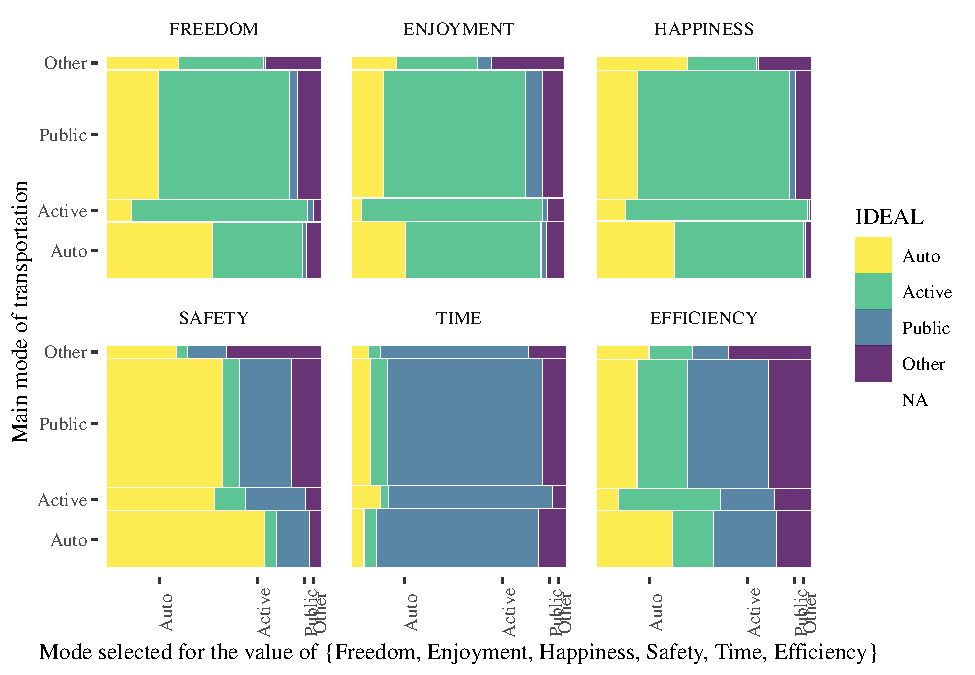
\includegraphics{Dissonance_Santiago_v1_files/figure-latex/figure-mosaic-plots-by-attribute-1.pdf}
\caption{\label{fig:mosaic-plots-by-attribute}Mosaic plots for affective
values; the y-axis is the proportion of respondents by main mode of
transportation, and the x-axis is the proportion of modes selected for
each value}
\end{figure}

\hypertarget{age-1}{%
\subsubsection{4.2.1 Age}\label{age-1}}

Words go here to discuss results by age.

\begin{figure}
\centering
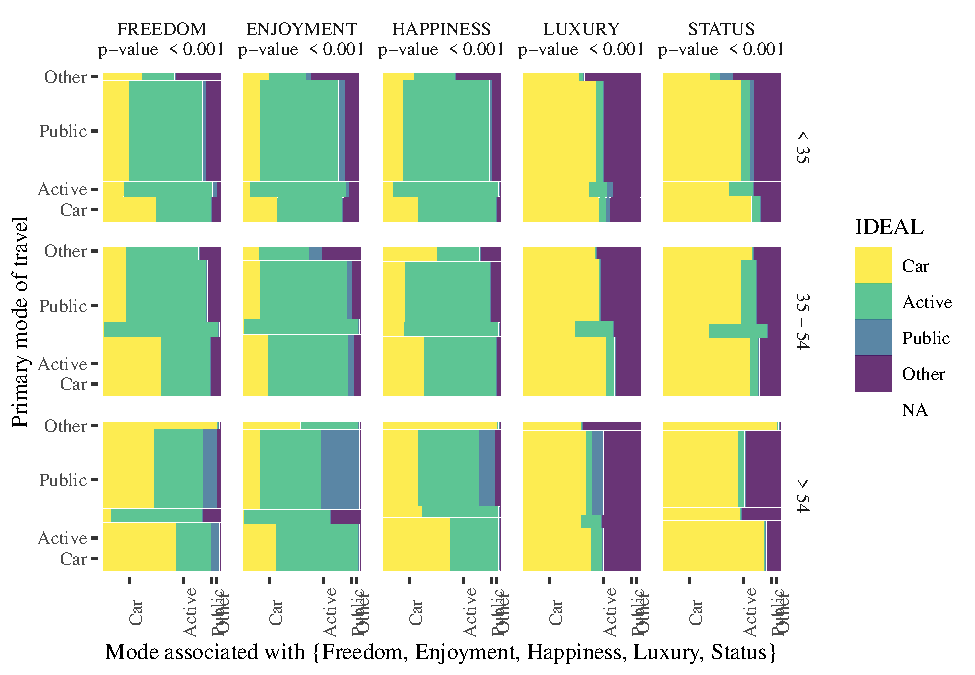
\includegraphics{Dissonance_Santiago_v1_files/figure-latex/figure-mosaic-plots-by-attribute-and-age-1.pdf}
\caption{\label{fig:mosaic-plots-by-age}Mosaic plots for affective
values by age; the y-axis is the proportion of respondents by main mode
of transportation, and the x-axis is the proportion of modes selected
for each value (p-values are for Cochran-Mantel-Haenszel Chi-Squared
Test)}
\end{figure}

\hypertarget{education-1}{%
\subsubsection{4.2.2 Education}\label{education-1}}

Words go here to discuss results by education.

\begin{figure}
\centering
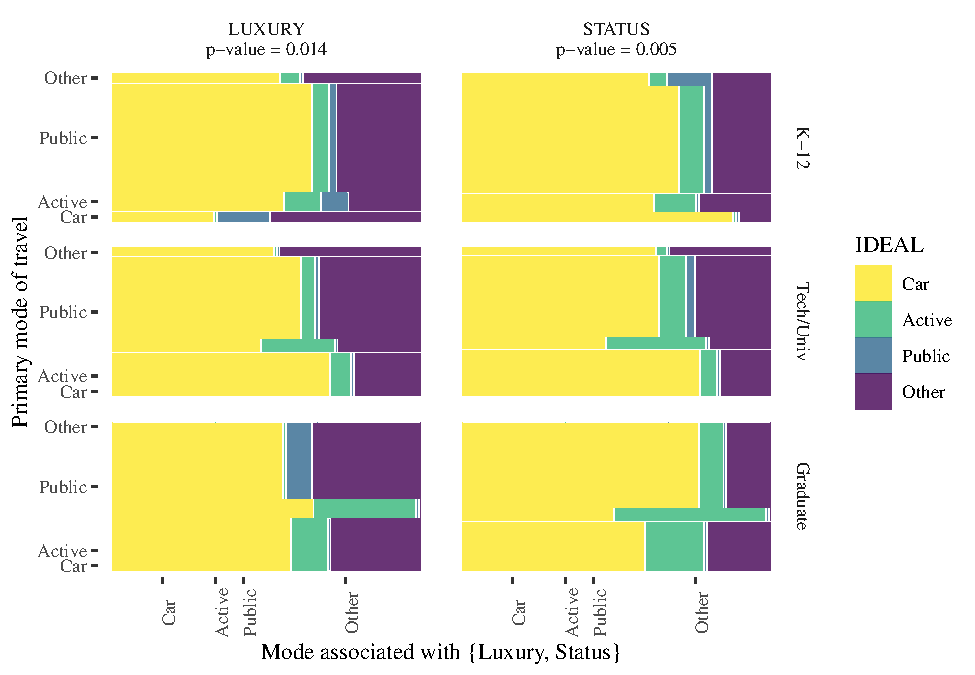
\includegraphics{Dissonance_Santiago_v1_files/figure-latex/figure-mosaic-plots-by-attribute-and-education-1.pdf}
\caption{\label{fig:mosaic-plots-by-education}Mosaic plots for affective
values by education; the y-axis is the proportion of respondents by main
mode of transportation, and the x-axis is the proportion of modes
selected for each value (p-values are for Cochran-Mantel-Haenszel
Chi-Squared Test)}
\end{figure}

\hypertarget{income-1}{%
\subsubsection{4.2.3 Income}\label{income-1}}

Words go here to discuss results by income.

\begin{figure}
\centering
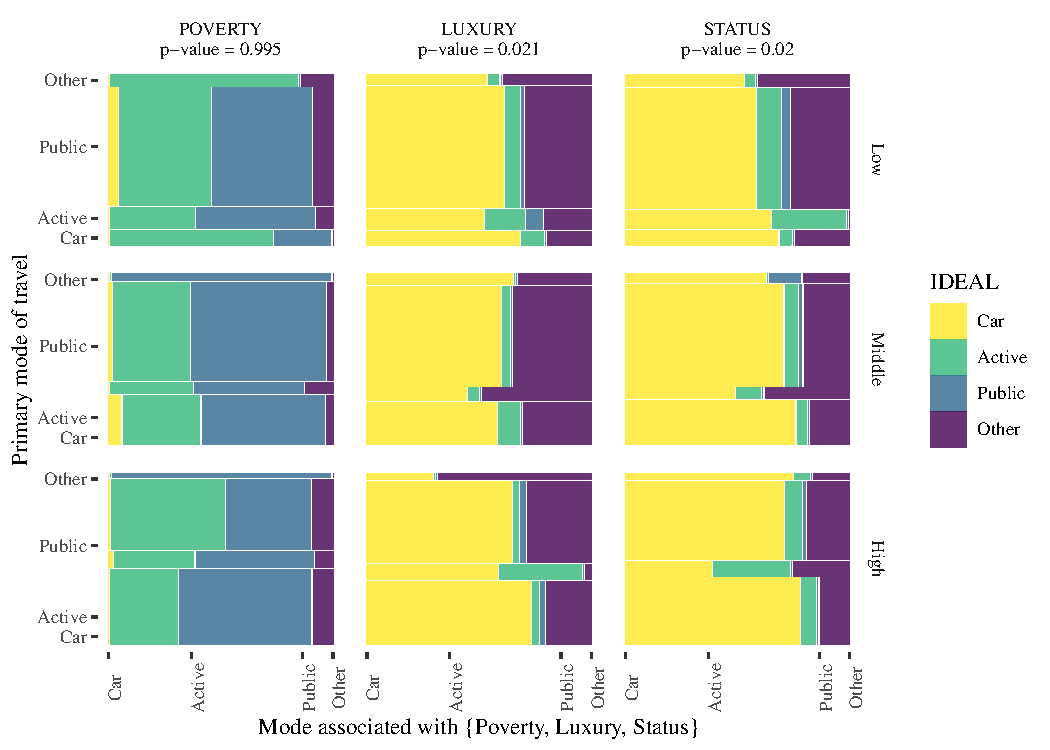
\includegraphics{Dissonance_Santiago_v1_files/figure-latex/figure-mosaic-plots-by-attribute-and-income-1.pdf}
\caption{\label{fig:mosaic-plots-by-income}Mosaic plots for affective
values by income; the y-axis is the proportion of respondents by main
mode of transportation, and the x-axis is the proportion of modes
selected for each value (p-values are for Cochran-Mantel-Haenszel
Chi-Squared Test)}
\end{figure}

\hypertarget{typical-commute-time-1}{%
\subsubsection{4.3.4 Typical commute
time}\label{typical-commute-time-1}}

Words go here to discuss results by time.

\begin{figure}
\centering
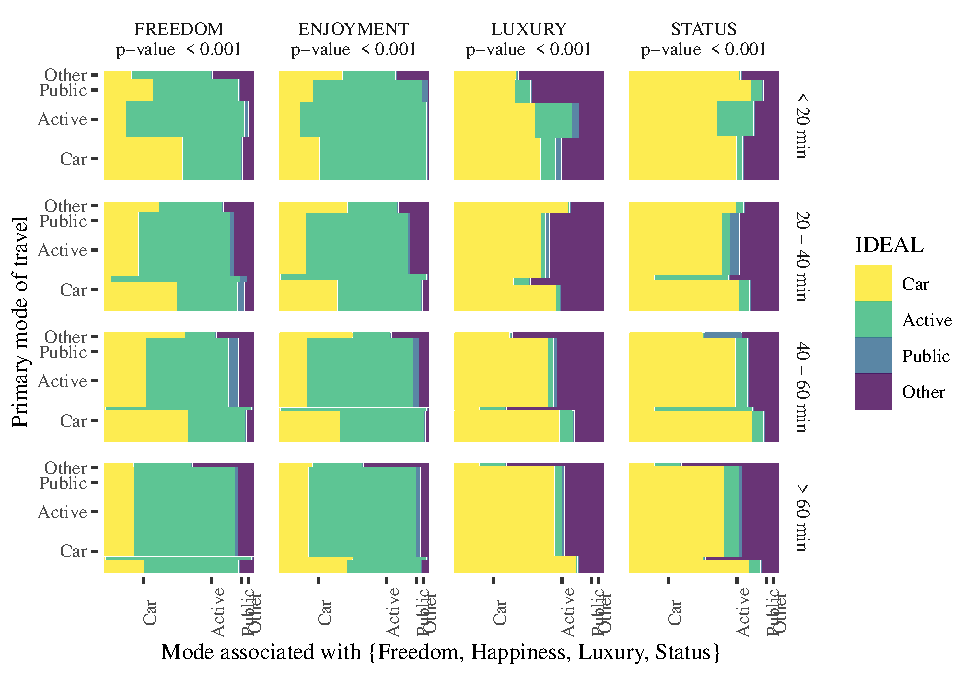
\includegraphics{Dissonance_Santiago_v1_files/figure-latex/figure-mosaic-plots-by-attribute-and-time-1.pdf}
\caption{\label{fig:mosaic-plots-by-travel-time}Mosaic plots for
affective values by commute time; the y-axis is the proportion of
respondents by main mode of transportation, and the x-axis is the
proportion of modes selected for each value (p-values are for
Cochran-Mantel-Haenszel Chi-Squared Test)}
\end{figure}

\textbf{\emph{FOR DISCUSSION}}

De Vos (2018)

\hypertarget{conclusions}{%
\section{5. Conclusions}\label{conclusions}}

Accordingly, the aim of this paper is to analyse some of the factors
that can potentially affect the levels of SWB in the wide spectrum of
public, private and active transport modes in the context of Santiago de
Chile. Previous research suggests that public transport users experience
a negative gap in desired and actual travel time, whereas active
travellers don't seem to mind somewhat longer trips than what strictly
needed (e.g., Páez and Whalen, 2010). In the context of a Latin American
country, historically the poor travel experience of public transit users
and active travellers reflects the social inequalities of social groups
that have no alternative but to move in these types of modes while
living far from the work centres and main activities. The paper aims to
reflect on the possibilities of increasing the SWB while travelling, and
how this could increase the attractiveness of public transport and
active travel in the socio-demographic groups studied. This can help not
only to reduce the use of private transport but also decrease the
inequality gap between these users.

The paper explores how positive affective and instrumental/utilitarian
factors of SWB correspond to the use of the primary mode of
transportation. It uses an analysis of correspondence that considers the
actual primary mode versus the mode that individuals associated to both
utilitarian (designed to be useful or practical rather than attractive)
and affective (expressing a person's feelings) SWB factors. For example,
it will be analysed if a person who uses public transport as the primary
mode, tends to associate these modes with positive affective factors (as
freedom, enjoyment or happiness) or positive utilitarian factors (as
security, time-savings or efficiency). We hypothesize that there is a
more persistent non-correspondence or mismatch within the more
disadvantage groups or within the users of public transport.

\hypertarget{acknowledgments}{%
\section{Acknowledgments}\label{acknowledgments}}

The following \texttt{R} packages were used in the course of this
investigation and the authors wish to acknowledge their developers:
\texttt{ggmosaic} (Jeppson et al., 2018), \texttt{ggthemes} (Arnold,
2018), \texttt{kableExtra} (Zhu, 2018), \texttt{knitr} (Xie, 2018,
2015), \texttt{rticles} (Allaire et al., 2018), and \texttt{tidyverse}
(Wickham, 2017).

\hypertarget{references}{%
\section*{References}\label{references}}
\addcontentsline{toc}{section}{References}

\hypertarget{refs}{}
\leavevmode\hypertarget{ref-Abenoza2017travel}{}%
Abenoza, R.F., Cats, O., Susilo, Y.O., 2017. Travel satisfaction with
public transport: Determinants, user classes, regional disparities and
their evolution. Transportation Research Part A: Policy and Practice 95,
64--84.

\leavevmode\hypertarget{ref-Alayyash2019commute}{}%
Al-Ayyash, Z., Abou-Zeid, M., 2019. Investigating commute satisfaction
differences of private car users and public transport users in a
developing country context. Transportation 46, 515--536.
doi:\href{https://doi.org/10.1007/s11116-019-10000-2}{10.1007/s11116-019-10000-2}

\leavevmode\hypertarget{ref-Allaire2018rticles}{}%
Allaire, J., Xie, Y., R Foundation, Wickham, H., Journal of Statistical
Software, Vaidyanathan, R., Association for Computing Machinery,
Boettiger, C., Elsevier, Broman, K., Mueller, K., Quast, B., Pruim, R.,
Marwick, B., Wickham, C., Keyes, O., Yu, M., Emaasit, D., Onkelinx, T.,
Gasparini, A., Desautels, M.-A., Leutnant, D., MDPI, Ögreden, O., Hance,
D., Nüst, D., 2018. Rticles: Article formats for r markdown.

\leavevmode\hypertarget{ref-Anable2005work}{}%
Anable, J., Gatersleben, B., 2005. All work and no play? The role of
instrumental and affective factors in work and leisure journeys by
different travel modes. Transportation Research Part A 39, 163--181.

\leavevmode\hypertarget{ref-Angotti1996latin}{}%
Angotti, T., 1996. Latin american urbanization and planning: Inequality
and unsustainability in north and south. Latin American Perspectives 23,
12--34.
doi:\href{https://doi.org/10.1177/0094582X9602300403}{10.1177/0094582X9602300403}

\leavevmode\hypertarget{ref-Argyle1999causes}{}%
Argyle, M., Kahneman, D., Diener, E., Schwarz, N., 1999. Causes and
correlates of happiness well-being: The foundations of hedonic
psychology.(pp. 353-373). New York, NY US: Russell Sage Foundation.

\leavevmode\hypertarget{ref-Arnold2018}{}%
Arnold, J.B., 2018. Ggthemes: Extra themes, scales and geoms for
'ggplot2'.

\leavevmode\hypertarget{ref-Bejarano2017user}{}%
Bejarano, M., Ceballos, L.M., Maya, J., 2017. A user-centred assessment
of a new bicycle sharing system in medellin. Transportation Research
Part F-Traffic Psychology and Behaviour 44, 145--158.
doi:\href{https://doi.org/10.1016/j.trf.2016.11.004}{10.1016/j.trf.2016.11.004}

\leavevmode\hypertarget{ref-Bergstad2011subjective}{}%
Bergstad, C.J., Gamble, A., Gärling, T., Hagman, O., Polk, M., Ettema,
D., Friman, M., Olsson, L.E., 2011. Subjective well-being related to
satisfaction with daily travel. Transportation 38, 1--15.

\leavevmode\hypertarget{ref-Bergstad2011affective}{}%
Bergstad, C.J., Gamble, A., Hagman, O., Polk, M., Garling, T., Olsson,
L.E., 2011. Affective-symbolic and instrumental-independence
psychological motives mediating effects of socio-demographic variables
on daily car use. Journal of Transport Geography 19, 33--38.
doi:\href{https://doi.org/10.1016/j.jtrangeo.2009.11.006}{10.1016/j.jtrangeo.2009.11.006}

\leavevmode\hypertarget{ref-Bocarejo2012transport}{}%
Bocarejo, S.J.P., Oviedo, H.D.R., 2012. Transport accessibility and
social inequities: A tool for identification of mobility needs and
evaluation of transport investments. Journal of Transport Geography 24,
142--154.
doi:\href{https://doi.org/10.1016/j.jtrangeo.2011.12.004}{10.1016/j.jtrangeo.2011.12.004}

\leavevmode\hypertarget{ref-Bornioli2019affective}{}%
Bornioli, A., Parkhurst, G., Morgan, P.L., 2019. Affective experiences
of built environments and the promotion of urban walking. Transportation
Research Part a-Policy and Practice 123, 200--215.
doi:\href{https://doi.org/10.1016/j.tra.2018.12.006}{10.1016/j.tra.2018.12.006}

\leavevmode\hypertarget{ref-Boschman2008toward}{}%
Boschmann, E.E., Kwan, M.P., 2008. Toward socially sustainable urban
transportation: Progress and potentials. International Journal of
Sustainable Transportation 2, 138--157.

\leavevmode\hypertarget{ref-Brown2009planning}{}%
Brown, J.R., Morris, E.A., Taylor, B.D., 2009. Planning for cars in
cities: Planners, engineers, and freeways in the 20th century. Journal
of the American Planning Association 75, 161--177.
doi:\href{https://doi.org/10.1080/01944360802640016}{10.1080/01944360802640016}

\leavevmode\hypertarget{ref-Cao2014satisfaction}{}%
Cao, X.Y., Ettema, D.F., 2014. Satisfaction with travel and residential
self-selection: How do preferences moderate the impact of the hiawatha
light rail transit line? Journal of Transport and Land Use 7, 93--108.
doi:\href{https://doi.org/10.5198/jtlu.v7i3.485}{10.5198/jtlu.v7i3.485}

\leavevmode\hypertarget{ref-Chapman2007transport}{}%
Chapman, L., 2007. Transport and climate change: A review. Journal of
Transport Geography 15, 354--367.
doi:\href{https://doi.org/10.1016/j.jtrangeo.2006.11.008}{10.1016/j.jtrangeo.2006.11.008}

\leavevmode\hypertarget{ref-Chatterjee2019commuting}{}%
Chatterjee, K., Chng, S., Clark, B., Davis, A., De Vos, J., Ettema, D.,
Handy, S., Martin, A., Reardon, L., 2019. Commuting and wellbeing: A
critical overview of the literature with implications for policy and
future research. Transport Reviews 30.
doi:\href{https://doi.org/10.1080/01441647.2019.1649317}{10.1080/01441647.2019.1649317}

\leavevmode\hypertarget{ref-Clark1996satisfaction}{}%
Clark, A.E., Oswald, A.J., 1996. Satisfaction and comparison income.
Journal of public economics 61, 359--381.

\leavevmode\hypertarget{ref-Delbosc2012role}{}%
Delbosc, A., 2012. The role of well-being in transport policy. Transport
Policy 23, 25--33.
doi:\href{https://doi.org/10.1016/j.tranpol.2012.06.005}{10.1016/j.tranpol.2012.06.005}

\leavevmode\hypertarget{ref-Devos2018people}{}%
De Vos, J., 2018. Do people travel with their preferred travel mode?
Analysing the extent of travel mode dissonance and its effect on travel
satisfaction. Transportation Research Part a-Policy and Practice 117,
261--274.
doi:\href{https://doi.org/10.1016/j.tra.2018.08.034}{10.1016/j.tra.2018.08.034}

\leavevmode\hypertarget{ref-Devos2019satisfaction}{}%
De Vos, J., 2019. Satisfaction-induced travel behaviour. Transportation
Research Part F-Traffic Psychology and Behaviour 63, 12--21.
doi:\href{https://doi.org/10.1016/j.trf.2019.03.001}{10.1016/j.trf.2019.03.001}

\leavevmode\hypertarget{ref-Devos2016travel}{}%
De Vos, J., Mokhtarian, P.L., Schwanen, T., Van Acker, V., Witlox, F.,
2016. Travel mode choice and travel satisfaction: Bridging the gap
between decision utility and experienced utility. Transportation 43,
771--796.

\leavevmode\hypertarget{ref-Devos2013travel}{}%
De Vos, J., Schwanen, T., Van Acker, V., Witlox, F., 2013. Travel and
subjective well-being: A focus on findings, methods and future research
needs. Transport Reviews 33, 421--442.
doi:\href{https://doi.org/10.1080/01441647.2013.815665}{10.1080/01441647.2013.815665}

\leavevmode\hypertarget{ref-Devos2015satisfying}{}%
De Vos, J., Schwanen, T., Van Acker, V., Witlox, F., 2015. How
satisfying is the scale for travel satisfaction? Transportation Research
Part F-Traffic Psychology and Behaviour 29, 121--130.
doi:\href{https://doi.org/10.1016/j.trf.2015.01.007}{10.1016/j.trf.2015.01.007}

\leavevmode\hypertarget{ref-Devos2019satisfying}{}%
De Vos, J., Schwanen, T., Van Acker, V., Witlox, F., 2019. Do satisfying
walking and cycling trips result in more future trips with active travel
modes? An exploratory study. International Journal of Sustainable
Transportation 13, 180--196.
doi:\href{https://doi.org/10.1080/15568318.2018.1456580}{10.1080/15568318.2018.1456580}

\leavevmode\hypertarget{ref-Devos2017travel}{}%
De Vos, J., Witlox, F., 2017. Travel satisfaction revisited. On the
pivotal role of travel satisfaction in conceptualising a travel
behaviour process. Transportation Research Part a-Policy and Practice
106, 364--373.
doi:\href{https://doi.org/10.1016/j.tra.2017.10.009}{10.1016/j.tra.2017.10.009}

\leavevmode\hypertarget{ref-Diener1997subjective}{}%
Diener, E., Eunkook Suh, M., 1997. Subjective well-being and age: An
international analysis. Annual review of gerontology and geriatrics 17,
304--324.

\leavevmode\hypertarget{ref-Domarchi2008effect}{}%
Domarchi, C., Tudela, A., Gonzalez, A., 2008. Effect of attitudes, habit
and affective appraisal on mode choice: An application to university
workers. Transportation 35, 585--599.
doi:\href{https://doi.org/10.1007/s11116-008-9168-6}{10.1007/s11116-008-9168-6}

\leavevmode\hypertarget{ref-Eriksson2013perceived}{}%
Eriksson, L., Friman, M., Gärling, T., 2013. Perceived attributes of bus
and car mediating satisfaction with the work commute. Transportation
Research Part A: Policy and Practice 47, 87--96.

\leavevmode\hypertarget{ref-Ettema2011satisfaction}{}%
Ettema, D., Garling, T., Eriksson, L., Friman, M., Olsson, L.E., Fujii,
S., 2011. Satisfaction with travel and subjective well-being:
Development and test of a measurement tool. Transportation Research Part
F-Traffic Psychology and Behaviour 14, 167--175.
doi:\href{https://doi.org/10.1016/j.trf.2010.11.002}{10.1016/j.trf.2010.11.002}

\leavevmode\hypertarget{ref-Ettema2010out}{}%
Ettema, D., Garling, T., Olsson, L.E., Friman, M., 2010. Out-of-home
activities, daily travel, and subjective well-being. Transportation
Research Part a-Policy and Practice 44, 723--732.
doi:\href{https://doi.org/10.1016/j.tra.2010.07.005}{10.1016/j.tra.2010.07.005}

\leavevmode\hypertarget{ref-Feldman1990settlement}{}%
Feldman, R.M., 1990. Settlement-identity: Psychological bonds with home
places in a mobile society. Environment and behavior 22, 183--229.

\leavevmode\hypertarget{ref-Ferrer2005income}{}%
Ferrer-i-Carbonell, A., 2005. Income and well-being: An empirical
analysis of the comparison income effect. Journal of public economics
89, 997--1019.

\leavevmode\hypertarget{ref-Friendly1994mosaic}{}%
Friendly, M., 1994. Mosaic displays for multi-way contingency tables.
Journal of the American Statistical Association 89, 190--200.

\leavevmode\hypertarget{ref-Friman2013psychometric}{}%
Friman, M., Fujii, S., Ettema, D., Gärling, T., Olsson, L.E., 2013.
Psychometric analysis of the satisfaction with travel scale.
Transportation Research Part A: Policy and Practice 48, 132--145.

\leavevmode\hypertarget{ref-Garling2019role}{}%
Garling, T., Bamberg, S., Friman, M., 2019. THE role of attitude in
choice of travel, satisfaction with travel, and change to sustainable
travel, Handbook of attitudes, vol 2: Applications, 2nd ed.

\leavevmode\hypertarget{ref-Gatersleben2007affective}{}%
Gatersleben, B., Uzzell, D., 2007. Affective appraisals of the daily
commute - comparing perceptions of drivers, cyclists, walkers, and users
of public transport. Environment and Behavior 39, 416--431.

\leavevmode\hypertarget{ref-Gossling2014sustainable}{}%
Gossling, S., Cohen, S., 2014. Why sustainable transport policies will
fail: EU climate policy in the light of transport taboos. Journal of
Transport Geography 39, 197--207.
doi:\href{https://doi.org/10.1016/j.jtrangeo.2014.07.010}{10.1016/j.jtrangeo.2014.07.010}

\leavevmode\hypertarget{ref-Handy2019commute}{}%
Handy, S., Thigpen, C., 2019. Commute quality and its implications for
commute satisfaction: Exploring the role of mode, location, and other
factors. Travel Behaviour and Society 16, 241--248.
doi:\href{https://doi.org/10.1016/j.tbs.2018.03.001}{10.1016/j.tbs.2018.03.001}

\leavevmode\hypertarget{ref-Hofmann2000exploring}{}%
Hofmann, H., 2000. Exploring categorical data: Interactive mosaic plots.
Metrika 51, 11--26.

\leavevmode\hypertarget{ref-Jeppson2019ggmosaic}{}%
Jeppson, H., Hofmann, H., Cook, D., 2018. Ggmosaic: Mosaic plots in the
'ggplot2' framework.

\leavevmode\hypertarget{ref-Khreis2016health}{}%
Khreis, H., Warsow, K.M., Verlinghieri, E., Guzman, A., Pellecuer, L.,
Ferreira, A., Jones, I., Heinen, E., Rojas-Rueda, D., Mueller, N.,
Schepers, P., Lucas, K., Nieuwenhuijsen, M., 2016. The health impacts of
traffic-related exposures in urban areas: Understanding real effects,
underlying driving forces and co-producing future directions. Journal of
Transport \& Health 3, 249--267.
doi:\href{https://doi.org/10.1016/j.jth.2016.07.002}{10.1016/j.jth.2016.07.002}

\leavevmode\hypertarget{ref-Lois2009relationship}{}%
Lois, D., Lopez-Saez, M., 2009. The relationship between instrumental,
symbolic and affective factors as predictors of car use: A structural
equation modeling approach. Transportation Research Part a-Policy and
Practice 43, 790--799.
doi:\href{https://doi.org/10.1016/j.tra.2009.07.008}{10.1016/j.tra.2009.07.008}

\leavevmode\hypertarget{ref-Lucas2012transport}{}%
Lucas, K., 2012. Transport and social exclusion: Where are we now?
Transport Policy 20, 107--115.
doi:\href{https://doi.org/10.1016/j.tranpol.2012.01.013}{10.1016/j.tranpol.2012.01.013}

\leavevmode\hypertarget{ref-Lucas2019evolution}{}%
Lucas, K., 2019. A new evolution for transport-related social exclusion
research? Journal of Transport Geography 102529.
doi:\href{https://doi.org/https://doi.org/10.1016/j.jtrangeo.2019.102529}{https://doi.org/10.1016/j.jtrangeo.2019.102529}

\leavevmode\hypertarget{ref-Martens2012justice}{}%
Martens, K., Golub, A., Robinson, G., 2012. A justice-theoretic approach
to the distribution of transportation benefits: Implications for
transportation planning practice in the united states. Transportation
research part A: policy and practice 46, 684--695.

\leavevmode\hypertarget{ref-Miller2011collaborative}{}%
Miller, H.J., 2011. Collaborative mobility: Using geographic information
science to cultivate cooperative transportation systems. Procedia -
Social and Behavioral Sciences 21, 24--28.
doi:\href{https://doi.org/http://dx.doi.org/10.1016/j.sbspro.2011.07.005}{http://dx.doi.org/10.1016/j.sbspro.2011.07.005}

\leavevmode\hypertarget{ref-Milne2012public}{}%
Milne, E.M.G., 2012. A public health perspective on transport policy
priorities. Journal of Transport Geography 21, 62--69.
doi:\href{https://doi.org/https://doi.org/10.1016/j.jtrangeo.2012.01.013}{https://doi.org/10.1016/j.jtrangeo.2012.01.013}

\leavevmode\hypertarget{ref-Mokhtarian2018travel}{}%
Mokhtarian, P.L., Pendyala, R.M., 2018. Travel satisfaction and
well-being, in: Friman, M., Ettema, D., Olsson, L.E. (Eds.), Quality of
Life and Daily Travel, Applying Quality of Life Research-Best Practices.
pp. 17--39.
doi:\href{https://doi.org/10.1007/978-3-319-76623-2_2}{10.1007/978-3-319-76623-2\_2}

\leavevmode\hypertarget{ref-Paez2010enjoyment}{}%
Paez, A., Whalen, K., 2010. Enjoyment of commute: A comparison of
different transportation modes. Transportation Research Part a-Policy
and Practice 44, 537--549.
doi:\href{https://doi.org/10.1016/j.tra.2010.04.003}{10.1016/j.tra.2010.04.003}

\leavevmode\hypertarget{ref-Pereira2017distributive}{}%
Pereira, R.H., Schwanen, T., Banister, D., 2017. Distributive justice
and equity in transportation. Transport reviews 37, 170--191.

\leavevmode\hypertarget{ref-Redman2013quality}{}%
Redman, L., Friman, M., Gärling, T., Hartig, T., 2013. Quality
attributes of public transport that attract car users: A research
review. Transport policy 25, 119--127.

\leavevmode\hypertarget{ref-Redmond2001positive}{}%
Redmond, L.S., Mokhtarian, P.L., 2001. The positive utility of the
commute: Modeling ideal commute time and relative desired commute
amount. Transportation 28, 179--205.

\leavevmode\hypertarget{ref-Schwanen2004extent}{}%
Schwanen, T., Mokhtarian, P.L., 2004. The extent and determinants of
dissonance between actual and preferred residential neighborhood type.
Environment and Planning B-Planning \& Design 31, 759--784.

\leavevmode\hypertarget{ref-Shao2019analysis}{}%
Shao, P., Liang, J., 2019. An analysis of the factors influencing the
sustainable use intention of urban shared bicycles in china.
Sustainability 11.
doi:\href{https://doi.org/10.3390/su11102721}{10.3390/su11102721}

\leavevmode\hypertarget{ref-Smith2017commute}{}%
Smith, O., 2017. Commute well-being differences by mode: Evidence from
portland, oregon, usa. Journal of Transport \& Health 4, 246--254.
doi:\href{https://doi.org/10.1016/j.jth.2016.08.005}{10.1016/j.jth.2016.08.005}

\leavevmode\hypertarget{ref-Steg2005car}{}%
Steg, L., 2005. Car use: Lust and must. Instrumental, symbolic and
affective motives for car use. Transportation Research Part A 39,
147--162.

\leavevmode\hypertarget{ref-Stlouis2014happy}{}%
St-Louis, E., Manaugh, K., Lierop, D. van, El-Geneidy, A., 2014. The
happy commuter: A comparison of commuter satisfaction across modes.
Transportation Research Part F-Traffic Psychology and Behaviour 26,
160--170.
doi:\href{https://doi.org/10.1016/j.trf.2014.07.004}{10.1016/j.trf.2014.07.004}

\leavevmode\hypertarget{ref-Susilo2014exploring}{}%
Susilo, Y.O., Cats, O., 2014. Exploring key determinants of travel
satisfaction for multi-modal trips by different traveler groups.
Transportation Research Part a-Policy and Practice 67, 366--380.
doi:\href{https://doi.org/10.1016/j.tra.2014.08.002}{10.1016/j.tra.2014.08.002}

\leavevmode\hypertarget{ref-Tesch2008gender}{}%
Tesch-Römer, C., Motel-Klingebiel, A., Tomasik, M.J., 2008. Gender
differences in subjective well-being: Comparing societies with respect
to gender equality. Social Indicators Research 85, 329--349.

\leavevmode\hypertarget{ref-Van2014effect}{}%
Van, H.T., Choocharukul, K., Fujii, S., 2014. The effect of attitudes
toward cars and public transportation on behavioral intention in
commuting mode choice-a comparison across six asian countries.
Transportation Research Part a-Policy and Practice 69, 36--44.
doi:\href{https://doi.org/10.1016/j.tra.2014.08.008}{10.1016/j.tra.2014.08.008}

\leavevmode\hypertarget{ref-Whalen2013mode}{}%
Whalen, K.E., Páez, A., Carrasco, J.A., 2013. Mode choice of university
students commuting to school and the role of active travel. Journal of
Transport Geography 31, 132--142.
doi:\href{https://doi.org/http://dx.doi.org/10.1016/j.jtrangeo.2013.06.008}{http://dx.doi.org/10.1016/j.jtrangeo.2013.06.008}

\leavevmode\hypertarget{ref-Wickham2017}{}%
Wickham, H., 2017. Tidyverse: Easily install and load the 'tidyverse'.

\leavevmode\hypertarget{ref-Xie2015}{}%
Xie, Y., 2015. Dynamic documents with r and knitr, 2nd ed. Chapman;
Hall/CRC, Boca Raton, Florida.

\leavevmode\hypertarget{ref-Xie2018}{}%
Xie, Y., 2018. Knitr: A general-purpose package for dynamic report
generation in r.

\leavevmode\hypertarget{ref-Ye2017satisfaction}{}%
Ye, R.N., Titheridge, H., 2017. Satisfaction with the commute: The role
of travel mode choice, built environment and attitudes. Transportation
Research Part D-Transport and Environment 52, 535--547.
doi:\href{https://doi.org/10.1016/j.trd.2016.06.011}{10.1016/j.trd.2016.06.011}

\leavevmode\hypertarget{ref-Zhu2018}{}%
Zhu, H., 2018. KableExtra: Construct complex table with 'kable' and pipe
syntax.

\leavevmode\hypertarget{ref-Zorrilla2019exploring}{}%
Zorrilla, M.C., Hodgson, F., Jopson, A., 2019. Exploring the influence
of attitudes, social comparison and image and prestige among
non-cyclists to predict intention to cycle in mexico city.
Transportation Research Part F-Traffic Psychology and Behaviour 60,
327--342.
doi:\href{https://doi.org/10.1016/j.trf.2018.10.009}{10.1016/j.trf.2018.10.009}


\end{document}


